\documentclass[11pt,a4paper]{article}

\usepackage[T1]{fontenc}
\usepackage[utf8]{inputenc}
\usepackage{lmodern}
\usepackage[margin=2.1cm]{geometry}
\usepackage{booktabs}
\usepackage{graphicx}
\usepackage{xcolor}
\usepackage{amsmath}
\usepackage{microtype}
\usepackage[hidelinks]{hyperref}
\usepackage{caption}
\usepackage{enumitem}
\usepackage{titlesec}
\usepackage{float}
\usepackage{tikz}
\usetikzlibrary{arrows.meta,positioning,fit,backgrounds,calc}

\captionsetup{font=small,labelfont=bf}
\titlespacing*{\section}{0pt}{1.1em}{0.45em}
\titlespacing*{\subsection}{0pt}{0.8em}{0.3em}
\setlist{nosep,leftmargin=1.3em}
\newcommand{\unit}[1]{\,\textsf{\small #1}}

\definecolor{callout}{RGB}{242,242,245}
\definecolor{box1}{RGB}{225,236,246}
\definecolor{box2}{RGB}{252,240,218}
\definecolor{box3}{RGB}{228,242,230}
\newcommand{\keybox}[1]{%
  \par\vspace{0.35em}\noindent\colorbox{callout}{%
  \begin{minipage}{\dimexpr\linewidth-2\fboxsep}\small #1\end{minipage}}\vspace{0.35em}\par}

\title{\vspace{-1.5cm}\textbf{DustCast}\\[0.2em]
\large A multi-scale forecasting service for Tunisian rooftop solar production,\\
with calibrated uncertainty and an evaluated model-selection loop}
\author{PESTGM 7.0 CDC Tech Challenge --- Track 1}
\date{September 2026}

\begin{document}
\maketitle
\vspace{-0.9cm}

\keybox{\textbf{What this is.} A forecasting service for rooftop PV production
at district, governorate and national scale, covering low- and medium-voltage
segments. It produces J+0 to J+7, has measured error at J+0 to J+3, quantifies
uncertainty, retrains and re-selects among five competing models each month from
observed forecast error, refreshes automatically when new weather arrives, and
exposes a documented HTTP API with a working downstream consumer.
\textbf{What we validated.} Accuracy and interval coverage were measured on real
PV production in Alice Springs, Australia. Suitable installation-level Tunisian
data were not available to this project, so Tunisian accuracy is unvalidated and
the Tunisian fleet is an explicit simulation. \textbf{What we found.} Model
selection matters more than model sophistication: a boosted model that wins on
the array it was developed on loses on arrays it has not seen, so the service
selects among models on held-back data rather than committing to one.}

\section{The service}

Tunisia has roughly 500\unit{MW} of residential rooftop PV and a further
$\sim$130\unit{MW} on medium- and high-voltage networks. This generation is
behind the meter and weather-driven, so the operator carries more reserve than
necessary and is exposed to ramps it could have anticipated.

\begin{figure}[H]
\centering
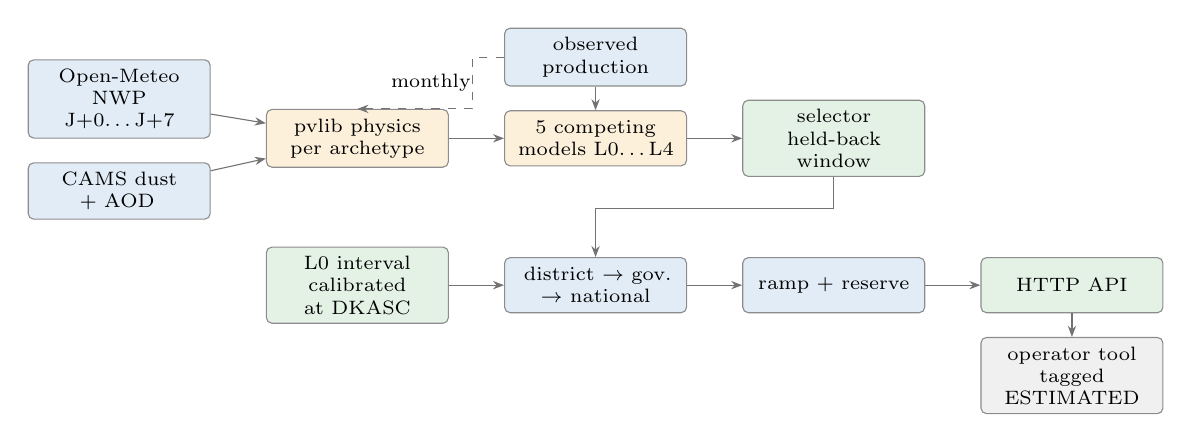
\begin{tikzpicture}[
  font=\scriptsize,
  box/.style={draw=black!45, rounded corners=2pt, align=center,
              minimum height=7mm, inner xsep=3pt, text width=21mm},
  a/.style={box, fill=box1}, b/.style={box, fill=box2}, c/.style={box, fill=box3},
  ar/.style={-{Stealth[length=4pt]}, draw=black!55}]

% --- row 1: weather in, models, selection
\node[a] (nwp) {Open-Meteo NWP\\J+0\dots J+7};
\node[a, below=3mm of nwp] (dust) {CAMS dust + AOD};
\node[b, right=7mm of nwp, yshift=-5mm] (phys) {pvlib physics\\per archetype};
\node[b, right=7mm of phys] (cand) {5 competing\\models L0\dots L4};
\node[a, above=3mm of cand] (obs) {observed\\production};
\node[c, right=7mm of cand] (sel) {selector\\held-back window};

% --- row 2: uncertainty, aggregation, delivery
\node[c, below=10mm of phys] (unc) {L0 interval\\calibrated at DKASC};
\node[a, right=7mm of unc] (agg) {district $\to$ gov.\\$\to$ national};
\node[a, right=7mm of agg] (dec) {ramp + reserve};
\node[c, right=7mm of dec] (api) {HTTP API};
\node[box, fill=black!6, below=3mm of api] (cons) {operator tool\\tagged\\ESTIMATED};

\draw[ar] (nwp) -- (phys); \draw[ar] (dust) -- (phys);
\draw[ar] (phys) -- (cand); \draw[ar] (obs) -- (cand);
\draw[ar] (cand) -- (sel);
\draw[ar] (sel.south) -- ++(0,-4mm) -| (agg.north);
\draw[ar] (unc) -- (agg);
\draw[ar] (agg) -- (dec); \draw[ar] (dec) -- (api);
\draw[ar] (api) -- (cons);
\draw[ar, dashed] (obs.west) -- ++(-4mm,0) |- node[pos=0.25, left, xshift=1mm]
  {monthly} (phys.north);
\end{tikzpicture}
\caption{Architecture. Solid path is a forecast request; the dashed path is the
learning loop, which refits every candidate monthly on past observations. The
operator workflow runs left to right: new weather lands $\to$ the service
rebuilds $\to$ models are scored and one is selected $\to$ the forecast is
aggregated and banded $\to$ a ramp and reserve view is derived $\to$ a
downstream tool reads it over HTTP, carrying the provenance flags with it.}
\end{figure}

\begin{table}[H]
\centering\small
\begin{tabular}{@{}lll@{}}
\toprule
\textbf{Capability} & \textbf{Implemented} & \textbf{Evidence in this report} \\
\midrule
District / governorate / national & 266 / 24 / 1 & Fig.~3, \S\ref{sec:assump} \\
LV and MV rooftop segments & 3 segments, 630\unit{MW} & Table~\ref{tab:seg} \\
Intra-day and J+1\dots J+3 & produced J+0\dots J+7 & Table~\ref{tab:hz} (J+0\dots J+3 only) \\
Learning from observed error & monthly refit + select & Fig.~2, Table~\ref{tab:replay} \\
Automatic refresh & on new weather, not a timer & \S\ref{sec:api} \\
Uncertainty & L0 band + aggregation & Table~\ref{tab:cov}, Fig.~3 \\
Machine exchange & 9 endpoints + consumer & \S\ref{sec:api} \\
\bottomrule
\end{tabular}
\caption{Every row is supported by a figure, table or section below.}
\end{table}

\section{Method}

\subsection{Physics first, learning on a capacity-normalised residual}

A \texttt{pvlib} model chain computes the power an array should produce from
forecast irradiance, temperature and wind given its geometry, capacity and age.
Models learn only the remainder. The target is \emph{normalised by AC inverter
capacity}:
\[
y_t \;=\; \frac{P^{\text{actual}}_t - P^{\text{expected}}_t}{P^{\text{AC}}_{\text{nom}}} .
\]

The normalisation is not cosmetic. The physics removes the diurnal and seasonal
\emph{shape} of production, but a residual expressed in kilowatts still scales
with array size. An earlier version of this work trained on kilowatts and
over-corrected small arrays by the capacity ratio, producing a positive bias at
every hour of the day. Dividing by capacity makes the target dimensionless, so it
can be learned on one array and spent on another.

Capacities are reported consistently as \emph{DC module} / \emph{AC inverter}:
array 3 is 4.95\unit{kW} DC on a 6.0\unit{kW} AC inverter; arrays 16C and 16D
are 1.98\unit{kW} DC on 2.5\unit{kW} AC. Normalisation and all nMAE denominators
use AC.

\subsection{Five competing models, and the loop that chooses between them}

\begin{table}[H]
\centering\small
\begin{tabular}{@{}llp{8.4cm}@{}}
\toprule
& \textbf{Model} & \textbf{Fitted from} \\
\midrule
L0 & physics & site geometry only --- requires \emph{no} local production data \\
L1 & + fitted derate & one scalar: mean actual/expected \\
L2 & + diurnal bias & thirteen numbers: mean residual by local hour \\
L3 & + boosted & XGBoost on the normalised residual \\
L4 & + diurnal, then boosted & L2 first, XGBoost on what L2 leaves behind \\
\bottomrule
\end{tabular}
\caption{These compete; this is not a progression in which more data eventually
promotes the machine-learned model.}
\end{table}

At each monthly boundary every candidate is \textbf{refitted} on past data only
--- the boosted models are retrained, not re-ranked --- the best performer on a
held-back 42-day window that no model was fitted on is selected, and that choice
forecasts the following month blind. Updating parameters from observed error is
the learning loop; reordering a leaderboard would not be.

\section{Results}

\subsection{Accuracy by horizon}

Forecasts are issued from the model run of the stated lead day and are valid for
the labelled hour: J+1 means a run issued one day before the valid time. All
models are fitted before 2025-03-30 and scored after.

\begin{table}[H]
\centering\small
\begin{tabular}{@{}lrrrrr@{}}
\toprule
\textbf{Valid horizon} & \textbf{L0} & \textbf{L1} & \textbf{L2} & \textbf{L3} & \textbf{L4} \\
\midrule
J+0 (same-day run) & 5.57 & 4.93 & 3.90 & 3.10 & \textbf{2.93} \\
J+1 & 6.67 & 5.57 & 4.42 & \textbf{4.23} & 4.36 \\
J+2 & 6.70 & 5.68 & 4.52 & \textbf{3.72} & 4.44 \\
J+3 & 6.74 & 5.72 & 4.67 & \textbf{3.78} & 3.97 \\
\bottomrule
\end{tabular}
\caption{nMAE (\%) of AC capacity, 1{,}251 daylight hours, DKASC array 3.
\textbf{Not an independent result}: array 3 is the array on which the feature set
and hyperparameters were chosen. Day-block bootstrap intervals for the best ML
model against L2 exclude zero at every horizon (J+0 $+24.7\%$, J+1 $+4.3\%$,
J+2 $+17.6\%$, J+3 $+19.0\%$), which is consistent with those choices having been
fitted to this array. \S\ref{sec:gen} tests the same models on arrays never seen.}
\label{tab:hz}
\end{table}

Error does not increase monotonically from J+1 to J+3 --- J+2 scores better than
J+1. We report the ordering as observed and draw no conclusion from it: there is
no requirement that empirical error rise with lead time, and we ran no test on
the horizon-to-horizon differences. J+0 is a same-day model run, not a nowcast;
the service has no sub-hourly or sky-imagery input and claims no minute-scale
skill.

\subsection{What the learning loop did}

\begin{figure}[H]
\centering
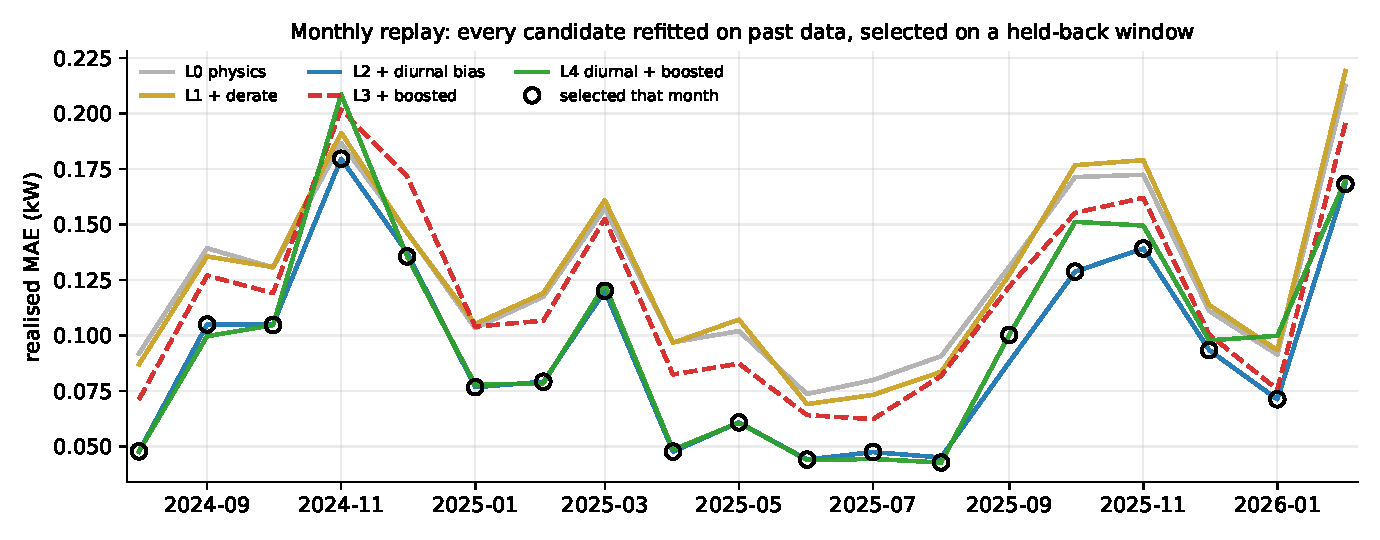
\includegraphics[width=\linewidth]{fig_replay.pdf}
\caption{Nineteen months of replay on array 16C. Every candidate is refitted on
past data at each boundary; the circled point is the model selected for that
month, chosen on a held-back window \emph{before} the month began.}
\end{figure}

\begin{table}[H]
\centering\small
\begin{tabular}{@{}lr@{\hskip 2em}lrr@{}}
\toprule
\textbf{Selection} & & \textbf{Model} & \textbf{Pooled nMAE} & \textbf{vs.\ selector} \\
\midrule
L2 selected & 14 / 19 & \textbf{selector (the service)} & \textbf{3.916\,\%} & --- \\
L4 selected & 5 / 19 & L2 + diurnal bias & 3.897\,\% & $-0.48\,\%$ \\
Switches & 7 & L4 diurnal + boosted & 4.162\,\% & $+5.9\,\%$ \\
Selection was month's winner & 12 / 19 & L3 + boosted & 4.827\,\% & $+18.9\,\%$ \\
\textbf{An ML model won the month} & \textbf{8 / 19} & L0 physics & 5.154\,\% & $+24.0\,\%$ \\
\bottomrule
\end{tabular}
\caption{Pooled over all 19 months, weighted by hours. The service achieved
3.916\,\% nMAE. The single best fixed choice in hindsight, L2, achieved
3.897\,\% --- the service was \textbf{0.019 percentage points worse, or 0.48\,\%
in relative terms}. It beat every other fixed choice, including both boosted
models. A switching policy is not bounded below by the best fixed model in
general; here it landed just short of one and well ahead of the rest.}
\label{tab:replay}
\end{table}

The machine-learned model is competitive rather than decorative: it won outright
in 8 of 19 months and was selected in 5. It trails on the pooled figure because
its losing months are the heavy ones --- an asymmetric error profile, not uniform
inferiority.

\subsection{Uncertainty, and what it covers}

The national layer runs L0 (\S\ref{sec:tunisia}), so its interval must be built
for L0. We calibrate a split-conformal band on arrays that \emph{have} measured
production, as a fraction of AC capacity, binned by sun elevation and clear-sky
index --- both known at forecast time. Half-width at 90\,\% nominal is 0.146 of
AC capacity overall, widening under cloud (0.161--0.168 for clear-sky index
0.4--0.7) and narrowing in clear high sun (0.101 above 45\textdegree).

\begin{table}[H]
\centering\small
\begin{tabular}{@{}lrrrr@{}}
\toprule
\textbf{Array} & \textbf{azimuth} & \textbf{hours} & \textbf{PICP} & \textbf{PINAW} \\
\midrule
DKASC 3 & 0\textdegree & 1{,}272 & 94.1\,\% & 0.259 \\
DKASC 16C & 90\textdegree & 3{,}269 & 92.1\,\% & 0.245 \\
DKASC 16D & 280\textdegree & 1{,}347 & 86.4\,\% & 0.240 \\
\bottomrule
\end{tabular}
\caption{Out-of-sample coverage of the L0 band, calibrated on 11{,}246 daylight
hours before 2025-03-30 and scored after. Nominal 90\,\%. Coverage and sharpness
are reported together: either alone is gameable, since a band from zero to
infinity has perfect coverage and no value.}
\label{tab:cov}
\end{table}

Regional bands are aggregated with
$\sqrt{\left(1+(n-1)\rho\right)/n}$, which recovers the plain sum at $\rho=1$ and
the $\sqrt{n}$ reduction at $\rho=0$. We estimate $\rho=0.485$ as the mean
pairwise correlation of the forecast clear-sky index across the 24 governorates,
giving a factor of 0.711 at $n=24$. At the modelled national peak this is
$\pm$72.3\unit{MW} on 454.4\unit{MW}, against 101.7\unit{MW} if errors were
assumed perfectly correlated and 20.8\unit{MW} if independent.

\keybox{\textbf{What Table~\ref{tab:cov} does and does not establish.} It
establishes the L0 band's coverage at three Australian sites, out of sample. It
does \emph{not} establish national coverage over Tunisia. Aggregating calibrated
site bands does not calibrate the aggregate: that depends on $\rho$, which is
estimated from forecast clear-sky index and never checked against a measured
national series, because none was available to this project. Tunisian site
coverage is likewise unvalidated.}

\subsection{Generalisation across arrays}
\label{sec:gen}

Having revised models, baselines and calibration while inspecting one window, we
froze the pipeline and evaluated it on array 16C --- a different array, east
facing rather than north, 1.98\unit{kW} DC rather than 4.95, over a later period.

\begin{table}[H]
\centering\small
\begin{tabular}{@{}llrr@{}}
\toprule
\textbf{Stage} & \textbf{Configuration} & \textbf{Skill vs.\ L2} & \textbf{95\,\% CI} \\
\midrule
\emph{(i)} initial frozen evaluation & as frozen & $-46.8\,\%$ & $[-53.7, -41.0]$ \\
\emph{(ii)} after correcting a degenerate ageing fit & post-hoc & $-48.3\,\%$ & $[-55.3, -42.2]$ \\
\emph{(iii)} capacity-normalised target & post-hoc & $-23.1\,\%$ & \\
\emph{(iv)} \quad + site bias adaptation & post-hoc & $-15.6\,\%$ & \\
\midrule
fresh array 16D (west), 2 training azimuths & post-hoc & $-9.4\,\%$ & $[-12.1, -7.0]$ \\
\bottomrule
\end{tabular}
\caption{Only \emph{(i)} is a frozen-protocol result. Everything below it was
introduced \emph{after} inspecting that result --- the ageing fit was degenerate
and was repaired, the unit error was found and fixed, and the site-bias variant
was added to give the boosted model the same site adaptation the L2 baseline
receives. Refitting those on earlier dates does not undo the fact that the
changes were test-informed. They are diagnostics of \emph{why} the model failed
to transfer, not independent confirmations that it now does.}
\end{table}

The pattern is consistent: the boosted model wins on the array it was developed
on (Table~\ref{tab:hz}) and loses on arrays it has not seen. That is the
signature of overfitting to a site. It is also why the service selects among
models rather than committing to one, and why the selector --- not the boosted
model --- is the contribution we claim.

\subsection{Operational implications, under a stated scenario}

The forecast is only useful if it changes a decision. To show what it would
change, we combine the simulated fleet with an assumed evening-peaking demand
shape peaking at 4{,}600\unit{MW}. \textbf{Everything in this subsection is an
output of those assumptions, not a measurement of the Tunisian grid}; the
assumptions are listed in Table~\ref{tab:seg}. We report it because the shape of
the answer --- where in the day rooftop PV actually matters to an operator --- is
robust to the exact numbers in a way the magnitudes are not.

\begin{figure}[H]
\centering
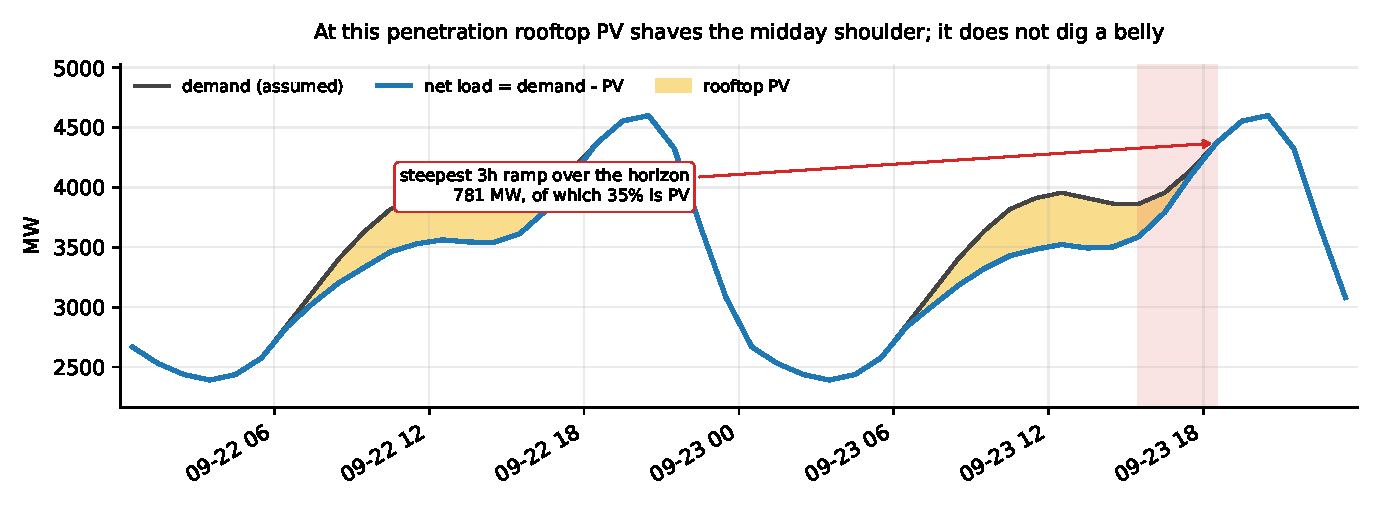
\includegraphics[width=\linewidth]{fig_netload.pdf}
\caption{Two modelled days of national net load, under the assumed demand shape
and simulated fleet of \S\ref{sec:assump}. \textbf{These are scenario outputs,
not measurements of the Tunisian grid.}}
\end{figure}

Under that scenario, rooftop PV removes about 9.9\,\% of midday net load without
creating a midday minimum --- the system trough remains overnight --- and PV
falling away accounts for 281\unit{MW} of the steepest 787\unit{MW} three-hour
evening ramp. If the real fleet and demand resemble these assumptions, roughly a
third of the evening ramp is the component a production forecast can anticipate.

A reserve-procurement simulation over the same scenario gave a 3.6\,\% reduction
in forecast-sensitive decision cost for a boosted forecast over L2, but at
\emph{lower achieved reliability} (unserved energy 65.9 against
36.0\unit{MWh}), and the sign of the saving reverses across plausible cost
assumptions (range $-9.9\,\%$ to $+6.4\,\%$ over twenty cases). We therefore
report it as inconclusive. Separately, using a fixed 90\,\% display interval
directly as a reserve policy performed poorly ($-41.1\,\%$ against the baseline,
$-46.4\,\%$ against the same model's scalar band); the narrow conclusion is about
that policy, not about coverage-calibrated bands in general.

\section{Deployment assumptions and sources}
\label{sec:assump}

\begin{table}[H]
\centering\small
\begin{tabular}{@{}llp{6.1cm}@{}}
\toprule
\textbf{Quantity} & \textbf{Value used} & \textbf{Basis and status} \\
\midrule
Residential rooftop & 500\unit{MW} (LV) & STEG statement, end-June 2026. The Ministry has separately cited ``$\sim$400\unit{MW} installed vs.\ 70\unit{MW} operational''; we flag the conflict rather than resolving it \\
Commercial / services & 78\unit{MW} (LV-MV) & \textbf{our split} of the $\sim$130\unit{MW} MV/HV figure \\
Industrial & 52\unit{MW} (MV) & \textbf{our split}, as above \\
Capacity by governorate & population-weighted & \textbf{assumption}; real PROSOL uptake is unlikely to be proportional to population \\
Aggregation units & 266, from delegation counts & \textbf{prototype units} --- see below \\
Tilt / azimuth / size mix & per-segment distributions & \textbf{assumption}; no registry was available to fit them \\
Demand shape and peak & 4{,}600\unit{MW} evening-peaking & \textbf{assumption} for the scenario in \S3.5 \\
\bottomrule
\end{tabular}
\caption{Every entry in bold is ours, not a published figure.}
\label{tab:seg}
\end{table}

\textbf{On aggregation units.} We subdivide each governorate into as many units
as it has delegations, and treat those as prototype aggregation units. We have
\emph{not} established that they correspond to the operational units STEG would
want, which are more likely defined by network topology --- HV/MV substations and
MV feeders --- than by administrative boundaries. The intended mapping is a
lookup from each installation's connection point to its feeder and substation,
replacing the administrative split without changing the aggregation code, which
sums whatever units it is given. Unit \emph{names} are not modelled.

\textbf{On weather resolution.} All units within a governorate currently share
one weather series. This is a modelling simplification we chose to keep the
service to 24 grid requests, \emph{not} a limit imposed by the data: an
$\sim$11\unit{km} forecast grid resolves variation well inside a Tunisian
governorate, and finer sampling is a matter of more requests. CAMS dust at
$\sim$40\unit{km} is the coarser constraint.

\textbf{On data availability.} Suitable installation-level data were not
available to this project: we found no accessible per-site registry or
generation time series for Tunisian rooftop PV. This is a statement about what we
could obtain, not a claim that no such records exist --- ANME guidance describes
commissioning records and inverter production histories, which would materially
change what is possible here if accessible.

\section{Reproducibility}

Every number and figure is regenerated from scripts in the repository; no figure
is drawn from retyped values.

\begin{table}[H]
\centering\small
\begin{tabular}{@{}lll@{}}
\toprule
\textbf{Dataset} & \textbf{Identity} & \textbf{Use} \\
\midrule
DKASC array 3 & \texttt{70-Site\_DKA-M5\_A-Phase}, 4.95/6.0\unit{kW}, az.\ 0\textdegree & training, horizons \\
DKASC 16C & 1.98/2.5\unit{kW}, az.\ 90\textdegree & frozen evaluation, replay \\
DKASC 16D & 1.98/2.5\unit{kW}, az.\ 280\textdegree \emph{(fitted, unverified)} & fresh evaluation \\
Open-Meteo forecast & hourly, J+0\dots J+7 & live weather \\
Open-Meteo historical forecast & archived runs, leads 1,2,3,5,7 & horizon evaluation \\
Open-Meteo air quality & CAMS, \texttt{domains=cams\_global} & dust, AOD \\
\bottomrule
\end{tabular}
\caption{All sources are free and keyless. Alice Springs production spans
2008--2026 at 5-minute resolution, resampled hourly with bins relabelled to
their midpoint before solar geometry is evaluated.}
\end{table}

\textbf{Boundaries.} Horizon evaluation fits before 2025-03-30 and scores after
(1{,}251 hours). The replay runs 2024-08 to 2026-02, refitting monthly, selecting
on the 42 days before each boundary and scoring the month after. Interval
calibration uses 11{,}246 daylight hours before 2025-03-30 across three arrays;
coverage is scored after. Daylight is sun elevation $>5$\textdegree; all nMAE
denominators are AC inverter capacity.

\textbf{Commands.} Each script prints its own result table and writes a CSV to
\texttt{data/artifacts/}.

\begin{table}[H]
\centering\small
\begin{tabular}{@{}ll@{}}
\toprule
\textbf{Script} & \textbf{Produces} \\
\midrule
\texttt{step16\_replay.py} & the learning loop, Fig.~2 and Table~\ref{tab:replay} \\
\texttt{step17\_horizons.py} & accuracy by horizon, Table~\ref{tab:hz} \\
\texttt{step18\_district\_national.py} & district $\to$ governorate $\to$ national \\
\texttt{step21\_national\_uncertainty.py} & interval calibration and aggregation, Table~\ref{tab:cov} \\
\texttt{step19\_consumer.py} & API and downstream consumer, end to end \\
\texttt{step14\_frozen\_holdout.py} & the frozen evaluation, stage \emph{(i)} \\
\texttt{step15\_multiarray.py} & normalisation and multi-array diagnostics \\
\texttt{step20\_report\_figures.py} & every figure in this report \\
\bottomrule
\end{tabular}
\end{table}

\section{The operator interface}
\label{sec:api}

A forecast is only operationally useful if another system can consume it without
a human in between. The service therefore exposes the forecast, its uncertainty
and its evaluation record over HTTP, and we ship a consumer that exercises the
whole path --- connect, check provenance, read the series, observe the refresh
behaviour, derive ramp and reserve quantities, and write a handoff file.

\begin{figure}[H]
\centering
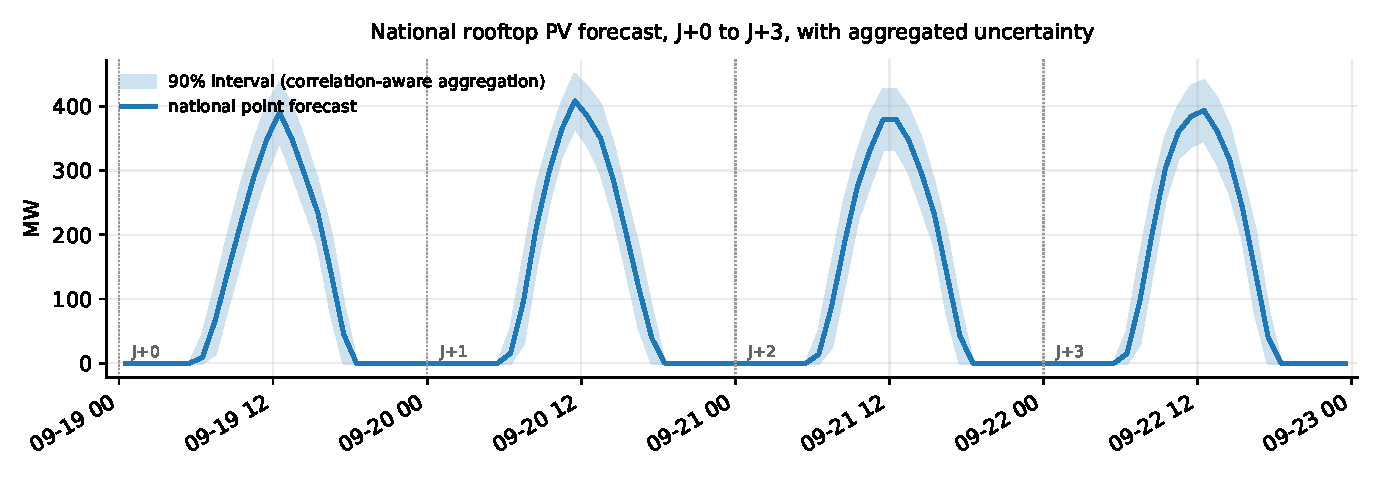
\includegraphics[width=\linewidth]{fig_forecast.pdf}
\caption{The product: national forecast with its aggregated 90\,\% interval
across J+0 to J+3, under the simulated fleet.}
\end{figure}

\begin{table}[H]
\centering\small
\begin{tabular}{@{}ll@{}}
\toprule
\textbf{Endpoint} & \textbf{Returns} \\
\midrule
\texttt{GET /health} & freshness, horizon length \\
\texttt{GET /meta} & scales, segments, capacity, provenance flags \\
\texttt{GET /forecast/national} & national MW series \\
\texttt{GET /forecast/governorate/\{key\}} & one governorate \\
\texttt{GET /forecast/governorates} & all 24, in the shape a map wants \\
\texttt{GET /forecast/district/\{key\}} & one unit, with its segment mix \\
\texttt{GET /models/performance} & measured nMAE by horizon \\
\texttt{GET /models/selection} & what the loop chose, month by month \\
\texttt{POST /refresh} & force a rebuild \\
\bottomrule
\end{tabular}
\caption{The evaluation record is served alongside the forecast, so a consumer
can see what the numbers are worth rather than having to trust them.}
\end{table}

\begin{verbatim}
$ curl -s localhost:8000/forecast/national | head
{ "generated_at": "2026-09-19T16:18:00+01:00", "rebuilt_on_this_request": false,
  "units": "MW (AC)", "model": "L0 physics",
  "fleet": "SIMULATED -- no installation registry available to this project",
  "evaluated_horizons": ["J+0","J+1","J+2","J+3"],
  "series": [ {"time": "2026-09-19T06:30:00+01:00", "mw": 12.4}, ... ] }
\end{verbatim}

Provenance travels with the numbers: a downstream tool that silently treated a
simulated national total as a metered one is the failure mode this interface
exists to prevent, and the sample consumer reads those flags and tags its output
\texttt{ESTIMATED}. Freshness is explicit, and a rebuild is triggered by new
weather arriving rather than by a timer.

\section{Limitations}

\begin{itemize}
\item \textbf{Tunisian accuracy is unvalidated.} The 5.57\,\% and 6.67\,\%
figures were measured at DKASC in Australia. No Tunisian production series was
available to score against.
\item \textbf{National interval coverage is unvalidated}, for the same reason;
only site coverage (Table~\ref{tab:cov}) is measured, and $\rho$ is estimated.
\item \textbf{The fleet is simulated}, including capacity allocation and segment
mix (Table~\ref{tab:seg}).
\item \textbf{Aggregation units are prototypes}, not verified STEG operational
units.
\item \textbf{The boosted model does not improve accuracy on unseen arrays}, and
is used only when selected.
\item \textbf{Scenario results in \S3.5} depend on an assumed demand shape and
fleet; they are not measurements of the Tunisian grid.
\item \textbf{Soiling has no ground truth} and is presented as a relative index
and maintenance trigger, never a measured loss.
\item \textbf{J+4 to J+7 are produced but not evaluated.}
\end{itemize}

\section{Conclusion}

DustCast is a working multi-scale rooftop PV forecasting service: district to
national, low- and medium-voltage segments, J+0 to J+7 produced with measured
error to J+3, calibrated intervals aggregated across regions, monthly retraining
and selection from observed forecast error, automatic refresh, and a documented
machine interface with a working consumer.

Its measured contribution is the selection loop. Five models compete; the service
achieved 3.916\,\% nMAE against 3.897\,\% for the best fixed choice identifiable
only in hindsight, and beat every other fixed choice by 6--24\,\%. That matters
because the ranking is not stable: the boosted model wins on the array it was
developed on and loses on arrays it has not seen, so a service that commits to
one model in advance is making a bet the evidence does not support.

The remaining gap is data, not method. Given installation-level Tunisian records
and any metered production, the same pipeline calibrates locally, the selector
has real candidates to choose between, and the coverage figures become Tunisian
rather than transferred.


\keybox{\textbf{Repository.}
\texttt{<<< INSERT REPOSITORY URL BEFORE SUBMISSION >>>} --- source, all
evaluation scripts, the API and the sample consumer. The DKASC production files
(313\unit{MB} and 285\unit{MB}) are not committed; the README gives the
\texttt{curl} commands that fetch them.}

\section*{Sources}
\small
\begin{enumerate}[label={[\arabic*]}]
\item STEG, statement on installed residential rooftop and MV/HV connected PV
capacity, end-June 2026 --- the 500\unit{MW} and $\sim$130\unit{MW} figures in
Table~\ref{tab:seg}. The Ministry has separately cited ``$\sim$400\unit{MW}
installed vs.\ 70\unit{MW} operational'' for low-voltage PV (Dec.\ 2025), which
appears to conflate registered pipeline with commissioned capacity; we flag the
conflict rather than resolving it.
\item IRENA, \emph{Renewable Capacity Statistics}, 2026 --- national PV fleet
$\sim$895\unit{MW}, for context.
\item ANME, guidance describing PROSOL installation commissioning records and
inverter production histories. Cited as evidence that installation-level records
are described as existing; we were unable to obtain an accessible dataset, which
is the limitation stated in \S\ref{sec:assump}.
\item Desert Knowledge Australia Solar Centre, Alice Springs, per-array 5-minute
production exports, \url{https://dkasolarcentre.com.au/download}.
\item Open-Meteo forecast, historical-forecast and air-quality APIs,
\url{https://open-meteo.com/en/docs}. Dust and AOD are CAMS-derived;
\texttt{domains=cams\_global} is required for Tunisian coverage.
\item Copernicus Atmosphere Monitoring Service (CAMS), global atmospheric
composition forecasts.
\item \texttt{pvlib python} --- Ineichen--Perez clear-sky, Hay--Davies
transposition, PVWatts DC and inverter models, SAPM cell temperature.
\item AEMO (Australia) and Sheffield Solar / Open Climate Fix (UK) --- the
sample-to-region upscaling method adopted in \S\ref{sec:assump}. Their samples
are metered; ours is simulated.
\item V.\ Vovk et al.\ and the split-conformal literature --- the finite-sample
quantile correction used for the L0 band in Table~\ref{tab:cov}.
\item M.\ Micheli et al., ``Impact of a Saharan dust outbreak on photovoltaics,''
\emph{Sustainable Energy Technologies and Assessments} 62 (2024) --- a March 2022
event halving the Spanish PV fleet's capacity factor for over two weeks.
\item \emph{Atmospheric Chemistry and Physics} 25:997 (2025) --- West African
dry-season dust reducing surface solar irradiance by $\sim$18\,\% on average.
With [10] this establishes mechanism and order of magnitude for dust impact,
\textbf{not} Tunisian values.
\item Decree 2016-1123 --- Tunisian net metering, capping surplus sales to STEG
at 30\,\% of annual production; relevant to self-consumption sizing in the fleet
assumptions.
\end{enumerate}

\end{document}